%%*****************************************************************************%%
%																				%
%																				%
%								LEAVE ME HERE									%
%																				%
%																				%
%              _____ ______   ________                   _______   				%  
%             |\   _ \  _   \|\   __  \                 /  ___  \    			%
%             \ \  \\\__\ \  \ \  \|\  \  ____________ /__/|_/  /|   			%
%              \ \  \\|__| \  \ \   _  _\|\____________\__|//  / /   			%
%               \ \  \    \ \  \ \  \\  \\|____________|   /  /_/__  			%
%                \ \__\    \ \__\ \__\\ _\                |\________\			%
%                 \|__|     \|__|\|__|\|__|                \|_______|			%
%                                                      							%
%																				%
%%*****************************************************************************%%
%									Links										%
%																				%
%		x Read only : https://www.overleaf.com/read/rbnmjbxzdcdw				%
%		x Edit&Read : https://www.overleaf.com/6933644zqzkpbnvzkwv				%
%		x Github	: https://www.github.com/MR-2								%
%																				%
%%*****************************************************************************%%
%							About - This Document								%
%																				%
%		x	 Pie Chart															%
%																				%
%		Note: Use it however you want.											%
%																				%
%%*****************************************************************************%%
%									Setup										%
%																				%
\documentclass[tikz,border=2mm]{standalone}
\usetikzlibrary{decorations.text}
									% Colors
\definecolor{LiUblue}{RGB}{0,185,231}
\definecolor{LiUturquoise}{RGB}{23,199,210}
\definecolor{LiUgreen}{RGB}{0,207,181}

\definecolor{LiUgreenx}{RGB}{91,202,236}
\definecolor{LiUturquoise2}{RGB}{101,207,216}
\definecolor{LiUgreen2}{RGB}{86,214,192}

\definecolor{LiUblue3}{RGB}{143,215,241}
\definecolor{LiUturquoise3}{RGB}{150,218,225}
\definecolor{LiUgreen3}{RGB}{143,223,207}

\definecolor{LiUblue4}{RGB}{189,230,246}
\definecolor{LiUturquoise4}{RGB}{194,231,236}
\definecolor{LiUgreen4}{RGB}{191,235,225}

\definecolor{LiUblue5}{RGB}{210,238,249}
\definecolor{LiUturquoise5}{RGB}{215,239,242}
\definecolor{LiUgreen5}{RGB}{213,241,235}

\definecolor{LiUorange}{RGB}{255,100,66}
\definecolor{LiUpurple}{RGB}{137,129,211}
\definecolor{LiUyellow}{RGB}{253,239,93}
\definecolor{LiUgray}{RGB}{106,126,145}

\definecolor{LiUorange3}{RGB}{255,164,154}
\definecolor{LiUpurple3}{RGB}{183,180,225}
\definecolor{LiUyellow3}{RGB}{254,244,165}
\definecolor{LiUgray3}{RGB}{170,178,187}

\definecolor{LiUorange5}{RGB}{255,220,216}
\definecolor{LiUpurple5}{RGB}{226,224,242}
\definecolor{LiUyellow5}{RGB}{254,250,220}
\definecolor{LiUgray5}{RGB}{221,224,227}

\definecolor{LiUhomepage}{RGB}{84,216,224}	



\newcommand{\drawsector}[6][]{
    \draw[#1] (#4:{#2-.5*#3}) arc [start angle = #4, delta angle=-#5, radius={#2-.5*#3}]--++({#4-#5}:#3) arc [start angle = {#4- #5}, delta angle=#5, radius={#2+.5*#3}] --cycle;
\draw[decorate,decoration={raise=-3pt, text along path, text=#6,text color=black, text align={align=center}}] (#4:#2) arc(#4:(#4-#5):#2);
}
\begin{document}
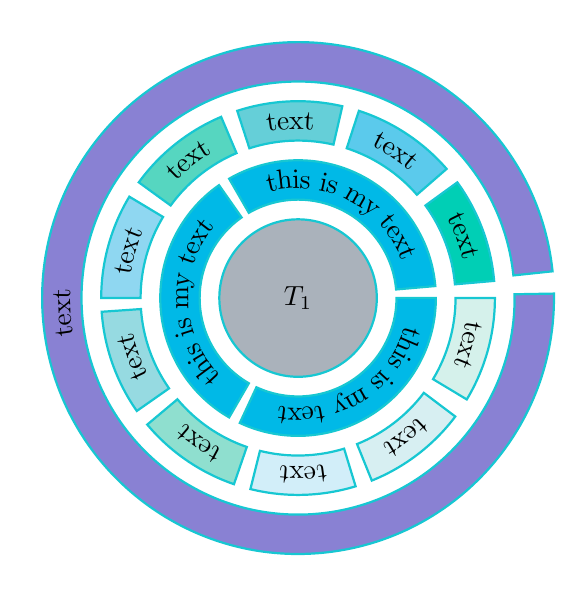
\begin{tikzpicture}   
%Center
\draw [draw=LiUturquoise, thick, fill=LiUgray3] (0,0) circle [radius=1] node {$T_1$};
%Second Circle
\drawsector[draw=LiUturquoise, thick, fill=LiUblue]{1.5}{0.5}{0}{115}{this is my text}
\drawsector[draw=LiUturquoise, thick, fill=LiUblue]{1.5}{0.5}{120}{115}{this is my text}
\drawsector[draw=LiUturquoise, thick, fill=LiUblue]{1.5}{0.5}{240}{115}{this is my text}
%Third Circle
\drawsector[draw=LiUturquoise, thick, fill=LiUgreen5]{2.25}{0.5}{0}{31}{text}
\drawsector[draw=LiUturquoise, thick, fill=LiUgreen]{2.25}{0.5}{36}{31}{text}
\drawsector[draw=LiUturquoise, thick, fill=LiUgreenx]{2.25}{0.5}{72}{31}{text}
\drawsector[draw=LiUturquoise, thick, fill=LiUturquoise2]{2.25}{0.5}{108}{31}{text}
\drawsector[draw=LiUturquoise, thick, fill=LiUgreen2]{2.25}{0.5}{144}{31}{text}
\drawsector[draw=LiUturquoise, thick, fill=LiUblue3]{2.25}{0.5}{180}{31}{text}
\drawsector[draw=LiUturquoise, thick, fill=LiUturquoise3]{2.25}{0.5}{215}{31}{text}
\drawsector[draw=LiUturquoise, thick, fill=LiUgreen3]{2.25}{0.5}{251}{31}{text}
\drawsector[draw=LiUturquoise, thick, fill=LiUblue5]{2.25}{0.5}{287}{31}{text}
\drawsector[draw=LiUturquoise, thick, fill=LiUturquoise5]{2.25}{0.5}{323}{31}{text}
%Fourth Circle
\drawsector[draw=LiUturquoise, thick, fill=LiUpurple]{3}{0.5}{1}{355}{text}

%\drawsector[draw=none, fill=blue!30]{2.5}{2}{180}{40}{text}
\end{tikzpicture}
%%*****************************************************************************%%
%																				%
%							 		  EOD   									%
%																				%
%%*****************************************************************************%%
\end{document}